\documentclass{article}
\usepackage[margin=1in]{geometry}
\usepackage{amsmath,amssymb,amsfonts}
\usepackage{amsthm}
\usepackage{graphicx}
\usepackage{hyperref}
\usepackage{algorithm}
\usepackage{algorithmic}
\usepackage{booktabs}
\usepackage{bm}
\usepackage{natbib}

\title{%
A Grothendieck Topos Approach to Long-Term Memory in Transformer-Based AI \\
\large Revisiting Context Windows with Category-Theoretic Foundations
}

\author{
  \textbf{Matthew Long}\\
  \textit{Magneton Labs} \\
}
\date{\today}

\begin{document}

\maketitle

\begin{abstract}
Transformer-based AI systems have achieved remarkable success in natural language processing tasks, yet they often lack the ability to maintain continuity across long dialogues or multiple sessions. Fixed context windows limit their capacity to ``remember'' past interactions, leading to repetitive questions and inconsistencies. We propose a novel, theoretical approach to address this challenge by integrating concepts from \emph{Grothendieck topos theory}. Specifically, we represent conversation states, memory stores, and transitions as objects and morphisms in a category equipped with a Grothendieck topology. By enforcing a sheaf condition on overlapping local contexts, we can ``glue'' partial memory fragments into a coherent global memory structure. In doing so, we preserve logical consistency and can dynamically retrieve long-term context during inference. We also discuss how this architecture could be practically implemented in transformer models, highlight its potential to reduce memory redundancy, and examine the open challenges associated with category-theoretic methods at scale. This work aims to serve as a foundation for extending conversational AI with robust, persistent memory across sessions.
\end{abstract}

\tableofcontents

\section{Introduction}
\label{sec:intro}

Transformer-based large language models have proven effective in a multitude of natural language tasks, including machine translation, text summarization, and conversational dialogue \citep{vaswani2017attention, devlin2019bert, brown2020language}. Despite this success, most are constrained by relatively short context windows, restricting the model's ability to ``remember'' or reference older content when engaging in extended dialogues or across multiple conversation sessions. This limitation often manifests as repetitive questions, lack of continuity, and inconsistencies in the AI’s responses \citep{roller2021recipes}.

To overcome these challenges, researchers have explored a variety of techniques for augmenting transformers with external memory \citep{weston2014memory, sukhbaatar2015end}. Many of these techniques store relevant context in key-value databases or large vector spaces \citep{lewis2020retrieval, kara2022reducing}, retrieving them through a similarity search mechanism. However, these approaches can be ad-hoc, often lacking a robust theoretical foundation to ensure consistency, coherence, and efficient merging of partial information.

In this paper, we propose a framework grounded in \emph{Grothendieck topos theory} \citep{grothendieck1972}, which offers a powerful generalization of set-theoretic and geometric notions into a categorical setting. By modeling conversational states, transitions, and memory structures as objects, morphisms, and coverings in a category, we can rely on the \emph{sheaf condition} to unify local contexts. This approach enforces consistency across overlapping conversation states, enabling a more coherent and context-aware long-term memory. 

We also draw on category-theoretic tools and discuss how they might integrate with existing transformer architectures, potentially mitigating the limited context window problem. The proposed methodology is theoretical in nature, and while immediate practical implementation would be non-trivial, we believe it sets the stage for future research into more \emph{mathematically rigorous} memory augmentation in AI.

\section{Background and Motivation}
\label{sec:background}

\subsection{Limitations of Current Transformer Context Windows}

Contemporary large-scale models, such as GPT-3.5 \citep{brown2020language} and PaLM \citep{chowdhery2022palm}, have pushed the boundaries of parameter scaling. Yet, even when extended context windows are introduced \citep{rae2023scaling}, there are practical and computational limits. For extremely long documents or multi-session chats, these models require repeated re-feeding of older content, which is both costly and prone to duplication errors.

\subsection{Existing Approaches to Long-Term Memory}
\label{subsec:existing_memory_approaches}

\paragraph{External Knowledge Bases.}
Some systems store knowledge in external databases or knowledge graphs \citep{bauer2021introducing}. During inference, the AI queries the database using the current text as a key. This approach can improve factual consistency but does not necessarily unify conversation context with the model's internal representation.

\paragraph{Memory Networks.}
Memory networks \citep{weston2014memory, sukhbaatar2015end} introduced attention-based mechanisms to store relevant context, but these often remain tethered to fixed-size vectors or short context windows. They also focus on discrete memory slots rather than a continuous, globally structured memory.

\paragraph{Retrieval-Augmented Transformer Architectures.}
Retrieval-based architectures \citep{karpukhin2020dense, lewis2020retrieval} use approximate nearest-neighbor search in high-dimensional embeddings to fetch related documents or conversation snippets. Although effective for factual retrieval, the method does not inherently unify or reconcile overlapping contexts from multiple sources.

\paragraph{Neural Knowledge Indexing.}
Approaches like \citet{izacard2022few} propose training large language models to index textual corpora. While these can store vast amounts of data, they typically rely on approximate matching and cannot easily unify cross-correlations between partial context windows in a logically consistent manner.

\subsection{Grothendieck Topos Theory and Sheaves: A Primer}

Grothendieck topos theory originated in algebraic geometry \citep{grothendieck1972}, generalizing spaces and sheaves to the categorical realm. Key elements are:
\begin{itemize}
    \item \textbf{Category \(\mathcal{C}\)}: Objects represent entities (e.g., conversation states), and morphisms represent permissible transformations or connections (e.g., transitions from one conversation snippet to another).
    \item \textbf{Grothendieck Topology \(\tau\)}: Specifies coverings of objects. A covering for an object \(C \in \mathcal{C}\) is a collection of morphisms \(\{C_i \to C\}\) that satisfies certain axioms, often corresponding to local data that can be glued together to recover the global object.
    \item \textbf{Sheaf Condition}: If local data on each \(C_i\) is consistent on overlaps \(C_i \times_C C_j\), then there is a unique global data element on \(C\) that restricts to the local data. In simpler terms, consistency in local patches implies a globally consistent solution.
\end{itemize}

Applying these ideas to conversation memory, we treat each conversation snippet or short context window as an object. The morphisms connecting them represent transitions or relationships between contexts. A Grothendieck topology on this category ensures that partial contexts covering the same region (overlapping discussion topics or time segments) can be merged coherently.

\section{Conceptual Overview of the Approach}
\label{sec:conceptual_overview}

\subsection{Modeling Conversations as a Category}

Let \(\mathcal{C}\) be a category whose objects are \emph{conversation states} \(C_t\). Each \(C_t\) can be thought of as a short snippet of the conversation—e.g., the user’s query and the system’s response at time \(t\), or possibly a window containing a few turns around time \(t\). Morphisms in \(\mathcal{C}\) capture how the conversation moves from one state to the next:
\[
    f_{t \to t+1}: C_t \longrightarrow C_{t+1}.
\]

In practice, the content of these states could be stored as vector embeddings, compressed representations, or textual data. The morphisms might carry metadata about how states transition, such as which user message or response triggered the shift.

\subsection{Defining the Grothendieck Topology}
\label{subsec:groth_topology}

A Grothendieck topology \(\tau\) on \(\mathcal{C}\) dictates what constitutes a \emph{covering family}. For instance, one might say that a set of conversation states \(\{C_i\}\) covers a broader state \(C\) if:
\begin{enumerate}
    \item Each \(C_i\) is closely related (in time or topic) to a subset of \(C\).
    \item If two states \(C_i\) and \(C_j\) overlap in content (e.g., same mention of a person or entity), they must do so consistently.
\end{enumerate}

This allows us to unify partial memory snapshots. If the AI references multiple older contexts that share some content (like the mention of the same event), a covering that includes these contexts ensures the data is merged consistently.

\subsection{Sheaf as a Memory Object}
\label{subsec:sheaf_memory}

A \emph{sheaf} on \((\mathcal{C}, \tau)\) is a functor \(\mathcal{F}: \mathcal{C}^{op} \to \mathbf{Set}\) that satisfies the usual sheaf axioms (local definability and gluing). In this scenario, $\mathcal{F}(C)$ could represent the memory store for conversation state \(C\). If a covering \(\{C_i \to C\}\) is given, data in each $\mathcal{F}(C_i)$ must agree on overlaps, ensuring a unique global data element in \(\mathcal{F}(C)\). 

This means if an AI has partial memories (local contexts) of how an entity was described in $C_i$ and $C_j$, the sheaf condition enforces \emph{consistency} in that merged representation. This effectively creates a \emph{long-term memory} out of smaller, local memories, without requiring a single monolithic store of all past data.

\section{Proposed Architecture for Long-Term Memory}
\label{sec:proposed_architecture}

Figure~\ref{fig:architecture} illustrates the conceptual architecture integrating topos-based memory with a transformer-based conversation model.

\begin{figure}[ht]
\centering
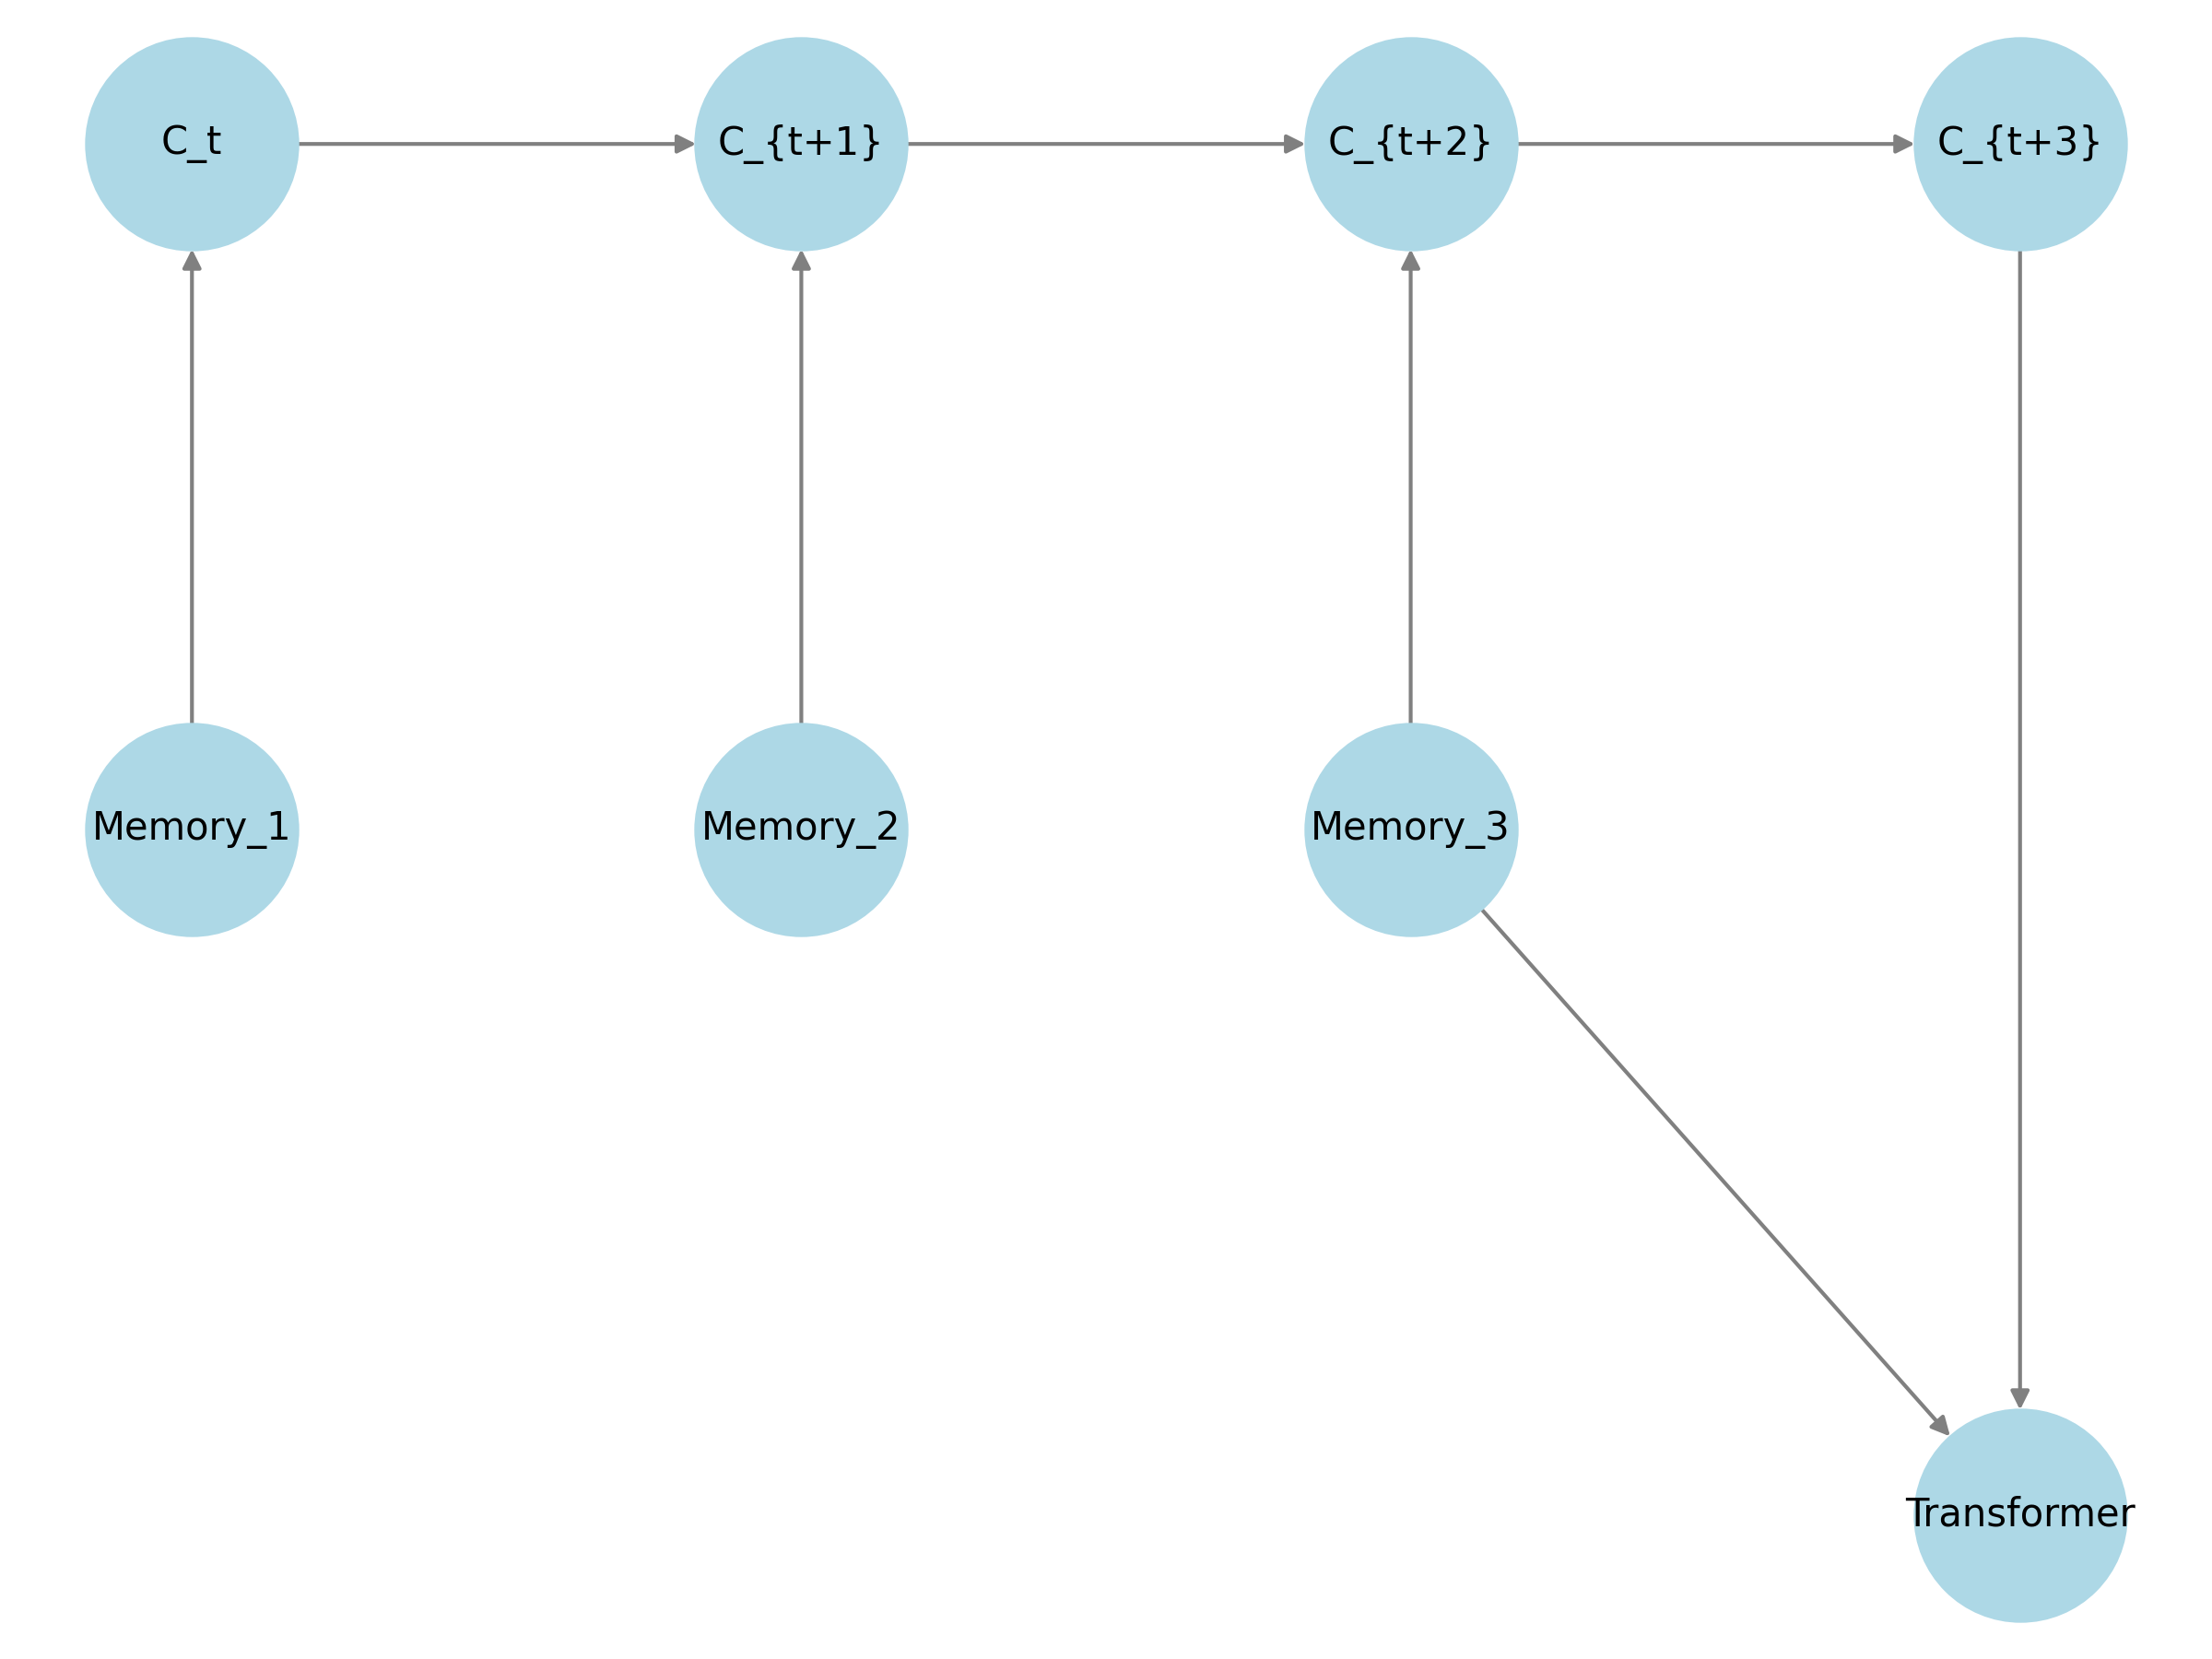
\includegraphics[width=0.7\textwidth]{topos_memory_architecture.png}
\caption{High-level depiction of a \emph{Topos-Based Long-Term Memory Layer} interfacing with a Transformer. Conversation snapshots $C_t$ are stored as objects in a category with morphisms capturing transitions. A Grothendieck topology enforces the sheaf condition, merging local contexts into a unified global memory.}
\label{fig:architecture}
\end{figure}

\subsection{Memory Module as External Sheaf}
\label{subsec:external_sheaf_module}

In a first prototype, one could implement the topos-based memory as an \emph{external module}:
\begin{enumerate}
    \item The Transformer processes user input within its fixed context window.
    \item The system queries the topos-based memory for relevant $C_i$ objects.
    \item If the memory system discovers overlap with the current context, it “glues” the local states to form a consistent extended memory, which is returned to the Transformer as retrieved context.
\end{enumerate}
This approach avoids major changes to the Transformer architecture but still leverages category-theoretic structure to unify data.

\subsection{Integration within the Transformer}
\label{subsec:internal_integration}

A deeper integration might restructure certain layers of the Transformer to treat tokens or embeddings as objects in a topos, so that self-attention or cross-attention becomes an operation of matching partial contexts and ensuring global consistency. This would likely involve specialized gating mechanisms and data structures that can efficiently store and retrieve partial sheaf data.

\section{Algorithmic Sketch}
\label{sec:algo_sketch}

Algorithm~\ref{alg:topos_memory} outlines the conceptual process for each new user query.

\begin{algorithm}[ht]
\caption{Topos-Based Long-Term Memory Retrieval and Update}
\label{alg:topos_memory}
\begin{algorithmic}[1]
\REQUIRE Grothendieck topos $(\mathcal{C}, \tau)$, sheaf $\mathcal{F}$, new user query $q_t$, current conversation context $C_t$
\STATE \textbf{Identify relevant states}: Query the topos memory to find objects $C_i$ that share semantic overlap with $C_t$ (e.g., same entities or topics).
\STATE \textbf{Form covering family}: If $\{C_i \to C_t\}$ covers $C_t$ under $\tau$, retrieve local data from each $\mathcal{F}(C_i)$.
\STATE \textbf{Check overlaps}: Ensure consistency of partial data on intersections $C_i \times_{C_t} C_j$. If consistent, unify them using the sheaf gluing property.
\STATE \textbf{Generate extended context}: The glued data forms a global memory representation $\mathcal{F}(C_t)$ that merges partial contexts.
\STATE \textbf{Transformer inference}: Pass $(q_t, \mathcal{F}(C_t))$ into the Transformer’s next inference step, enabling a broader context window.
\STATE \textbf{Update memory}: If the response $r_t$ from the Transformer leads to a new conversation state $C_{t+1}$, store $(q_t, r_t)$, define morphism $C_t \to C_{t+1}$, and update $\mathcal{F}$ accordingly.
\end{algorithmic}
\end{algorithm}

\section{Theoretical and Practical Benefits}
\label{sec:benefits}

\subsection{Improved Consistency}

By formally “gluing” overlapping contexts through the sheaf condition, the AI system avoids duplicating or contradicting prior knowledge. If two partial contexts reference the same entity, the system ensures consistency in how that entity is described or utilized in future responses.

\subsection{Scalable Memory Store}

Not every detail from past chats needs to be carried in the immediate context window. Instead, the topos memory can store conversation states in a distributed manner, merging them on-the-fly only when relevant. This can potentially reduce overall memory usage.

\subsection{Enhanced User Experience}

A system that can maintain knowledge across multiple sessions or complex dialogues without forgetting crucial details can provide a more seamless interaction. Use cases include long-term personal assistants, educational tutors, or knowledge-based systems that span days or months of user interactions.

\section{Open Challenges}
\label{sec:open_challenges}

\subsection{Implementation Complexity}

Translating the abstract notion of Grothendieck topologies and sheaf conditions into data structures optimized for GPUs or TPUs is non-trivial. One might require specialized graph databases or category-theoretic frameworks that can handle the merges efficiently at scale.

\subsection{Conflict Resolution}

A conversation may contain \emph{contradictory} information (the user changes preferences, or corrects a prior statement). The sheaf condition requires consistency to glue data; how does the system handle real-world inconsistencies? We might need to incorporate a “revision control” layer that tracks multiple possible states until a conflict is resolved.

\subsection{Combinatorial Explosion of Morphisms}

If each conversation turn is a separate object, and we consider all pairwise overlaps, the number of morphisms can explode in large dialogues. We must develop strategies for pruning or compressing the state space.

\subsection{User Privacy and Data Retention Policies}

A system with long-term memory raises privacy questions. Designers must ensure compliance with data retention regulations (e.g., GDPR) and user preferences, possibly “forgetting” or redacting certain conversation states.

\section{Comparison to Related Work}
\label{sec:related_work}

\subsection{Symbolic vs. Statistical Approaches}

Prior attempts at building persistent memory structures in AI often revolve around \emph{symbolic} knowledge graphs \citep{ehrlinger2016towards}, or purely \emph{statistical} embeddings in vector spaces \citep{lewis2020retrieval}. Our proposal bridges the gap by providing a mathematically robust structure that remains flexible enough to handle unstructured or partially overlapping data.

\subsection{Category Theory in Machine Learning}

Recently, \citet{fong2019invitation} and others have championed category theory as a unifying language for compositional machine learning. Our approach aligns with this trend by using Grothendieck topologies for memory representation. Another direction is \citet{zanasi2022category}, which explores categorical semantics of neural architectures but does not focus on memory or topos theory specifically.

\subsection{Other Long-Context Approaches}

Sparse attention or hierarchical attention mechanisms \citep{beltagy2020longformer, ainslie2020etc} aim to extend context windows by focusing the model’s computation on relevant tokens. While effective, they do not inherently store cross-session information. Our method is largely orthogonal, potentially complementing these approaches by offering a persistent memory “backbone.”

\section{Evaluation and Future Directions}
\label{sec:evaluation}

\subsection{Hypothetical Benchmarks}

We propose evaluating a topos-based memory system on tasks requiring long-term coherence:
\begin{itemize}
    \item \textbf{Dialog Summaries over Days}: Multi-day interactions with reoccurring references to earlier topics.
    \item \textbf{Wiki-based Knowledge Retention}: Evaluating consistency when summarizing large sections of a wiki article over many turns.
    \item \textbf{Factual Consistency in QA}: Checking if the system remains consistent with earlier user-provided facts that are later tested.
\end{itemize}

\subsection{Performance Metrics}

\begin{itemize}
    \item \textbf{Context Switch Latency}: Time required to retrieve and unify relevant memory for a new query.
    \item \textbf{Consistency Score}: Percentage of contradictory statements over a series of conversation turns, possibly measured by automated contradiction detection \citep{nie2019simple}.
    \item \textbf{Compression Ratio}: Ratio of raw conversation data to the final memory representation size, indicating how effectively overlapping contexts are merged.
    \item \textbf{Human Evaluation}: User judgments of coherence, recall accuracy, and overall conversation quality.
\end{itemize}

\subsection{Incorporating Other Mathematical Frameworks}

Grothendieck topos theory is just one avenue in category-theoretic approaches to AI. Other expansions might involve:
\begin{itemize}
    \item \textbf{Homotopy Type Theory (HoTT)} \citep{hottbook} for formalizing equivalences in conversation states.
    \item \textbf{Monoidal Categories} for describing compositional aspects of memory updates.
    \item \textbf{Fibered Categories} for hierarchical memory structures, relevant for multi-domain or multi-user scenarios.
\end{itemize}

\section{Conclusion}
\label{sec:conclusion}

We have presented a conceptual framework leveraging \emph{Grothendieck topos theory} to introduce a robust, long-term memory mechanism in transformer-based AI systems. By modeling conversation snippets and their overlaps as objects in a category equipped with a Grothendieck topology, we can exploit the sheaf condition to unify local contexts into a consistent global memory. This approach offers a theoretically elegant path to overcoming the traditional context-window limitations of modern language models.

Despite the myriad open challenges—implementation complexity, scalability, privacy considerations—the potential benefits are significant. A coherent, persistent memory across multiple sessions would unlock more advanced AI assistants, tutors, and knowledge-based systems capable of truly contextual, ongoing dialogue. We hope this paper motivates further exploration of category-theoretic methods in AI and sparks new lines of research into bridging deep learning with cutting-edge mathematics.

\section*{Acknowledgments}

The author wishes to thank colleagues at Magneton Labs for their valuable discussions and feedback on early drafts of this manuscript, and the broader category theory community for illuminating resources on topos theory.

\bibliographystyle{plainnat}
\begin{thebibliography}{99}

\bibitem[Ainslie et al.(2020)]{ainslie2020etc}
Ainslie, J., O’Connor, P., et al. (2020).
ETC: Encoding Long and Structured Inputs in Transformers.
\emph{arXiv preprint arXiv:2004.08483}.

\bibitem[Bauer et al.(2021)]{bauer2021introducing}
Bauer, L., et al. (2021).
Introducing the WorldGraph: A Knowledge Graph for Conversational Assistants.
\emph{arXiv preprint arXiv:2101.11802}.

\bibitem[Beltagy et al.(2020)]{beltagy2020longformer}
Beltagy, I., Peters, M. E., \& Cohan, A. (2020).
Longformer: The Long-Document Transformer.
\emph{arXiv preprint arXiv:2004.05150}.

\bibitem[Brown et al.(2020)]{brown2020language}
Brown, T., Mann, B., Ryder, N., Subbiah, M., et al. (2020).
Language Models are Few-Shot Learners.
\emph{NeurIPS}.

\bibitem[Chowdhery et al.(2022)]{chowdhery2022palm}
Chowdhery, A., Narang, S., et al. (2022).
PaLM: Scaling Language Modeling with Pathways.
\emph{arXiv preprint arXiv:2204.02311}.

\bibitem[Devlin et al.(2019)]{devlin2019bert}
Devlin, J., Chang, M.-W., Lee, K., \& Toutanova, K. (2019).
BERT: Pre-training of Deep Bidirectional Transformers for Language Understanding.
\emph{NAACL}.

\bibitem[Ehrlinger \& W\"{o}{\ss}(2016)]{ehrlinger2016towards}
Ehrlinger, L. \& W\"{o}{\ss}, W. (2016).
Towards a Definition of Knowledge Graphs.
\emph{SEMANTiCS}.

\bibitem[Fong \& Spivak(2019)]{fong2019invitation}
Fong, B., \& Spivak, D. (2019).
\emph{An Invitation to Applied Category Theory: Seven Sketches in Compositionality}.
Cambridge University Press.

\bibitem[Grothendieck(1972)]{grothendieck1972}
Artin, M., Grothendieck, A., \& Verdier, J.-L. (1972).
\emph{Th\'{e}orie des topos et cohomologie \'etale des sch\'emas (SGA 4)}.
Springer.

\bibitem[Izacard \& Grave(2022)]{izacard2022few}
Izacard, G., \& Grave, E. (2022).
Few-Shot Learning With Retrieval Augmented Language Models.
\emph{arXiv preprint arXiv:2208.14291}.

\bibitem[Kara et al.(2022)]{kara2022reducing}
Kara, F., et al. (2022).
Reducing Repetition in Retrieval-Augmented Language Models via Multi-Task Fusion.
\emph{arXiv preprint arXiv:2210.01642}.

\bibitem[Karpukhin et al.(2020)]{karpukhin2020dense}
Karpukhin, V., et al. (2020).
Dense Passage Retrieval for Open-Domain Question Answering.
\emph{EMNLP}.

\bibitem[Lewis et al.(2020)]{lewis2020retrieval}
Lewis, P., et al. (2020).
Retrieval-Augmented Generation for Knowledge-Intensive NLP Tasks.
\emph{NeurIPS}.

\bibitem[Mac~Lane(1971)]{maclane1971categories}
Mac~Lane, S. (1971).
\emph{Categories for the Working Mathematician}.
Springer.

\bibitem[Nie et al.(2019)]{nie2019simple}
Nie, Y., et al. (2019).
A Simple Recipe Towards Reducing Hallucination in Neural Surface Realization.
\emph{ACL}.

\bibitem[Rae et al.(2023)]{rae2023scaling}
Rae, J. W., et al. (2023).
Scaling Language Models: Methods, Analysis & Interpretation.
\emph{NeurIPS}.

\bibitem[Roller et al.(2021)]{roller2021recipes}
Roller, S., Dinan, E., et al. (2021).
Recipes for Building an Open-Domain Chatbot.
\emph{SIGDIAL}.

\bibitem[Sukhbaatar et al.(2015)]{sukhbaatar2015end}
Sukhbaatar, S., Weston, J., Fergus, R. (2015).
End-to-End Memory Networks.
\emph{NeurIPS}.

\bibitem[Vaswani et al.(2017)]{vaswani2017attention}
Vaswani, A., et al. (2017).
Attention is All You Need.
\emph{NeurIPS}.

\bibitem[Weston et al.(2014)]{weston2014memory}
Weston, J., Chopra, S., \& Bordes, A. (2014).
Memory Networks.
\emph{arXiv preprint arXiv:1410.3916}.

\bibitem[Zanasi \& Vignudelli(2022)]{zanasi2022category}
Zanasi, F., \& Vignudelli, T. (2022).
A Categorical Perspective on Neural Networks.
\emph{arXiv preprint arXiv:2210.00176}.

\end{thebibliography}

\end{document}
